\documentclass[tikz,border=2mm]{standalone} 
\usetikzlibrary{positioning, fit, arrows.meta}

\begin{document}
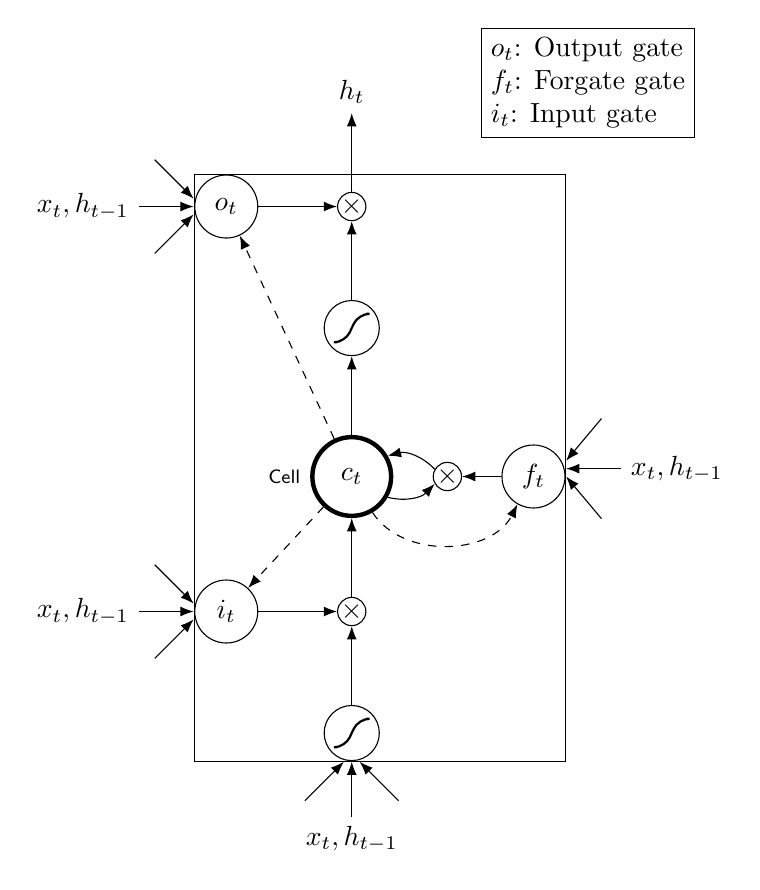
\begin{tikzpicture}[
    prod/.style={circle, draw, inner sep=0pt},
    ct/.style={circle, draw, inner sep=5pt, ultra thick, minimum width=10mm},
    ft/.style={circle, draw, minimum width=8mm, inner sep=1pt},
    filter/.style={circle, draw, minimum width=7mm, inner sep=1pt, path picture={\draw[thick, rounded corners] (path picture bounding box.center)--++(65:2mm)--++(0:1mm);
    \draw[thick, rounded corners] (path picture bounding box.center)--++(245:2mm)--++(180:1mm);}},
    mylabel/.style={font=\scriptsize\sffamily},
    >=LaTeX
    ]

\node[ct, label={[mylabel]left:Cell}] (ct) {$c_t$};
\node[filter, above=of ct] (int1) {};
\node[prod, above=of int1] (x1) {$\times$}; 
\node[above=of x1] (ht) {$h_t$};
\node[prod, below=of ct] (x2) {$\times$}; 
\node[filter, below=of x2] (int2) {};
\node[prod, right=5mm of ct] (x3) {$\times$}; 
\node[ft, right=5mm of x3] (ft) {$f_t$};
\node[ft, left=of x2] (it) {$i_t$};
\node[ft, left=of x1] (ot) {$o_t$};

\foreach \i/\j in {int2/x2, x2/ct, ct/int1, int1/x1,
            x1/ht, it/x2, ot/x1, ft/x3}
    \draw[->] (\i)--(\j);

\draw[->] (x3) to[bend right=30] (ct);
\draw[->] (ct) to[bend right=30] (x3);
\draw[dashed,->] (ct)--(ot);
\draw[dashed,->] (ct)--(it);
\draw[dashed,->] (ct) to[bend right=60] (ft);
\node[fit=(int2) (it) (ot) (ft), draw, inner sep=0pt] (fit) {};

\draw[<-] (fit.west|-it) coordinate (aux)--++(180:7mm) node[left]{$x_t,h_{t-1}$};
\draw[<-] ([yshift=1mm]aux)--++(135:7mm);
\draw[<-] ([yshift=-1mm]aux)--++(-135:7mm);

\draw[<-] (fit.west|-ot) coordinate (aux)--++(180:7mm) node[left]{$x_t,h_{t-1}$};
\draw[<-] ([yshift=1mm]aux)--++(135:7mm);
\draw[<-] ([yshift=-1mm]aux)--++(-135:7mm);

\draw[<-] (fit.south-|int2) coordinate (aux)--++(-90:7mm) node[below]{$x_t,h_{t-1}$};
\draw[<-] ([xshift=1mm]aux)--++(-45:7mm);
\draw[<-] ([xshift=-1mm]aux)--++(-135:7mm);

\draw[<-] (fit.east|-ft) coordinate (aux)--++(-50:7mm) ;
\draw[<-] ([yshift=1mm]aux)--++(0:7mm) node[right]{$x_t,h_{t-1}$};
\draw[<-] ([yshift=2mm]aux)--++(50:7mm);


\node[draw,align=left] at (3,5) {$o_t$: Output gate\\
$f_t$: Forgate gate\\
$i_t$: Input gate};

\end{tikzpicture}
\end{document}